\documentclass[CJKutf8,dvipsnames,table]{beamer}
\usepackage{hyperref}
\hypersetup{
  pdfpagemode={FullScreen},
  colorlinks={true},
  linkcolor={blue},
}

%% https://tex.stackexchange.com/questions/47576/combining-ifxetex-and-ifluatex-with-the-logical-or-operation
\usepackage{iftex}
\newif\ifxetexorluatex % a new conditional starts as false
\ifnum 0\ifxetex 1\fi\ifluatex 1\fi>0
   \xetexorluatextrue
\fi
\usepackage{ifplatform}
\ifxetexorluatex
	\usepackage[slantfont,boldfont]{xeCJK}
	\ifwindows
		\setCJKmainfont{SimSun} % Windows默认中文字体:中易宋体
	\else
		\ifmacosx
			\setCJKmainfont{STSong} % MacOS默认中文字体:华文宋体
		\else
			\setCJKmainfont{Noto Serif CJK SC} % Linux默认中文字体:思源宋体(By Adobe & Google)
		\fi
	\fi
\else
	\usepackage{CJKutf8}
\fi

\usepackage[export]{adjustbox}
\usepackage{mathptmx} %pdfTeX error: pdflatex (file fmex9.pfb): cannot open Type 1 font file for reading
                                                 %https://forum.ubuntu.com.cn/viewtopic.php?t=269943
\usepackage{mathtools}
\usepackage[mathscr]{urwchancal}

\usetheme{Madrid}%{Warsaw}
\usecolortheme{default}

\setbeamertemplate{footline}[page number]{} %gets rid of bottom navigation bars
\setbeamertemplate{navigation symbols}{} %gets rid of navigation symbols

\title{数字信号处理}
\subtitle{第6讲:采样与量化}
\author{洪明坚}
\institute{重庆大学软件学院}
\date{\today}

\begin{document}
\ifxetexorluatex\else
\begin{CJK*}{UTF8}{song}
\fi

  \AtBeginSection[]
  {
    \begin{frame}
      \frametitle{Outline}
      \tableofcontents[currentsection]
    \end{frame}
  }

  \frame{\titlepage}
  \frame{\frametitle{目录}\tableofcontents}
  
  \section{采样定理}
  
  %% PAGE
  \begin{frame}
    \frametitle{定义}
    \begin{itemize}
	\item 采样(sampling):把连续时间(CT)信号转换为离散时间(DT)信号
		\begin{itemize}
		\item 一般是等间距采样
		\end{itemize}
	\begin{center}
    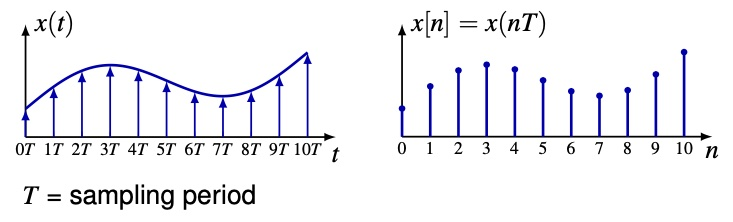
\includegraphics[scale=.4]{sampling}	
	\end{center}
    \end{itemize}
  \end{frame}    
   
  %% PAGE
  \begin{frame}
    \frametitle{定义}
    \begin{itemize}
	\item 采样会导致信息丢失
		\begin{itemize}
		\item 例如
		\[
			x_1(t)=cos(\frac{\pi}{3}t) {\color{red} \neq} x_2(t)=cos(\frac{7\pi}{3}t) 
		\]
		但是
		\[
			x_1[n]=cos(\frac{\pi}{3}n) {\color{red} =} x_2[n]=cos(\frac{7\pi}{3}[n])
		\]
		\end{itemize}
	\begin{center}
    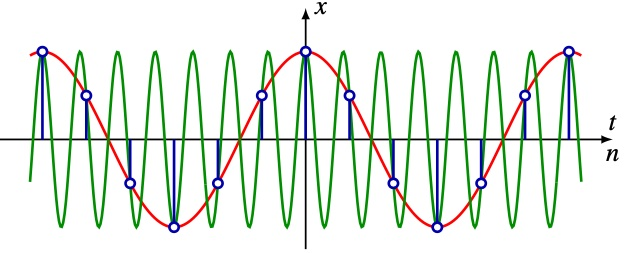
\includegraphics[scale=.4]{lossysampling}	
	\end{center}
	
	\item 问题:
		\begin{itemize}
		\item 什么条件下可以从采样中恢复信号?
		\item 如何恢复?
		\end{itemize}
    \end{itemize}
  \end{frame}   
     
  %% PAGE
  \begin{frame}
    \frametitle{冲激串采样}
    \begin{itemize}
    \item 时域
    \end{itemize}
    \begin{center}
      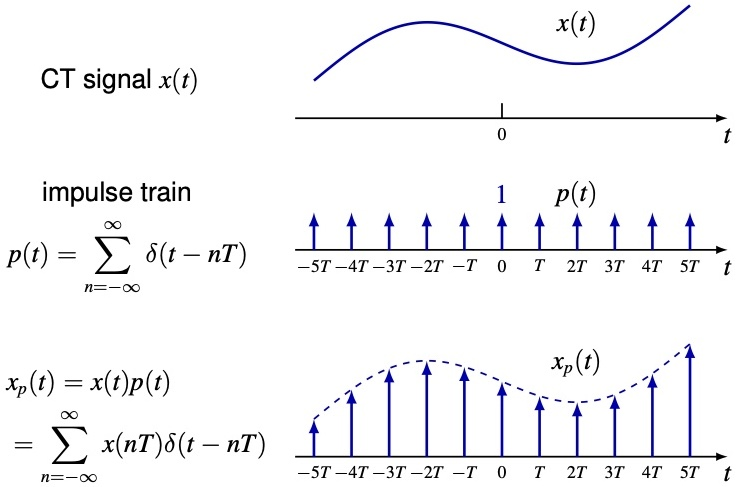
\includegraphics[scale=.4]{impulse-train-sampling-time}
    \end{center}
  \end{frame}  
  
  %% PAGE
  \begin{frame}
    \frametitle{冲激串采样}
    \begin{itemize}
    \item 频域
    \end{itemize}
    \begin{center}
      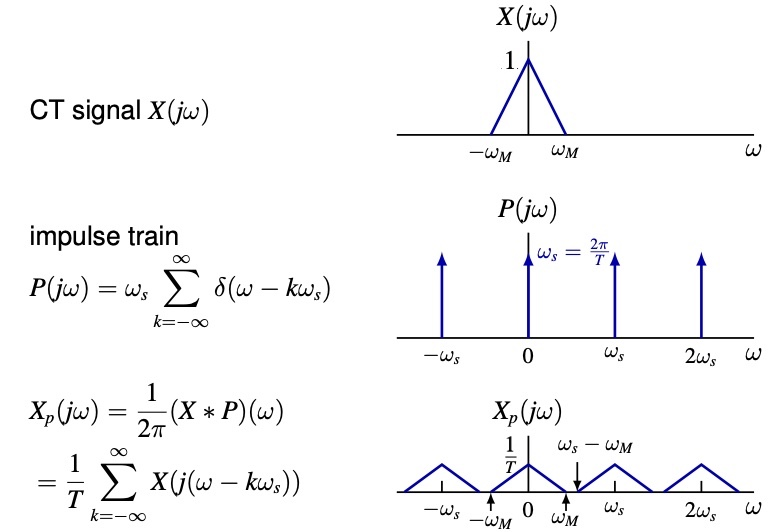
\includegraphics[scale=.4]{impulse-train-sampling-freq}
    \end{center}
  \end{frame}        

  %% PAGE
  \begin{frame}
    \frametitle{冲激串采样}
    \begin{itemize}
    \item 对于一个带限信号(banded-limit),即
    \[
    	X(j\omega) = 0, |\omega|>\omega_M
    \]
    用采样频率$\omega_s=\frac{2\pi}{T}$对它进行采样
    	\begin{itemize}
		\item 如果$\omega_s > 2\omega_M$,频谱没有重叠,可以用一个低通滤波器从$X_p(j\omega)$中恢复$X(j\omega)$
		\item 如果$\omega_s \leq 2\omega_M$,频谱出现重叠,则无法恢复
		\end{itemize}
    \end{itemize}
    \begin{center}
      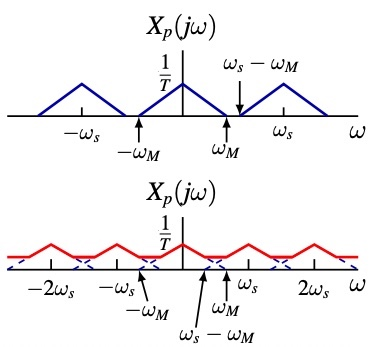
\includegraphics[scale=.4]{overlap}
    \end{center}
  \end{frame}   
     
  %% PAGE
  \begin{frame}
    \frametitle{采样定理}

	\begin{block}{奈奎斯特(Nyquist)采样定理(1928年)}
		设$x(t)$是某一个带限信号,在$|\omega|>\omega_M$时,$X(j\omega)=0$。
		如果$\omega_s{\color{red}>}2\omega_M$,其中$\omega_s=2\pi/T$,那么$x(t)$就唯一地由其样本
		$x(nT), n=0, \pm1, \pm2, \hdots$所确定。
		一般称$2\omega_M$为奈奎斯特采样频率。
	\end{block}

    \begin{center}
      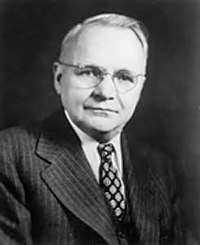
\includegraphics[scale=.5]{Harry_Nyquist} \\
      \href{https://en.wikipedia.org/wiki/Harry_Nyquist}{Harry Nyquist}      
    \end{center}
  \end{frame}  
       
  %% PAGE
  \begin{frame}
    \frametitle{采样定理}
	\begin{block}{重建方法}
		产生一个周期冲激串,其冲激幅度就是这些依次而来的采样值;然后将该冲激串通过一个增益为$T$、
		截止频率$\omega_c$满足$\omega_M < \omega_c < (\omega_s-\omega_M)$的理想低通滤波器,
		该滤波器的输出就是$x(t)$。
	\end{block}
    \begin{center}
      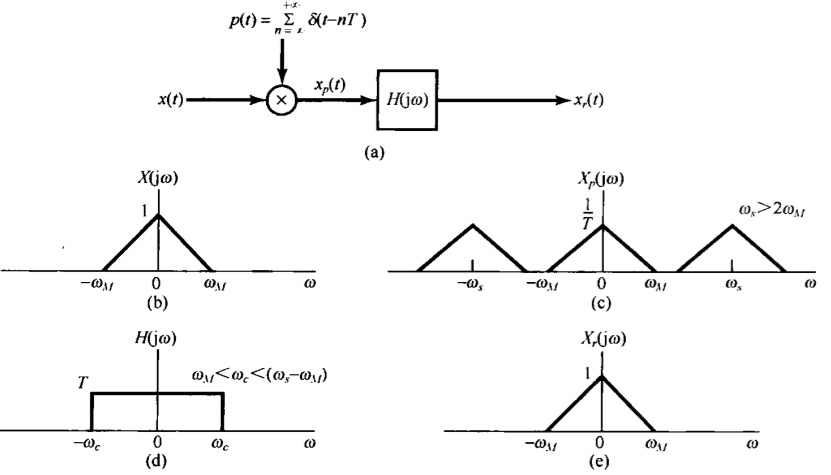
\includegraphics[scale=.3]{ss-c-f7-4}
    \end{center}
  \end{frame} 
         
  %% PAGE
  \begin{frame}
    \frametitle{Questions}
    \begin{itemize}
    \item Any questions?
    \end{itemize}
    \begin{center}
      
\includegraphics[scale=.5]{question}
    \end{center}
  \end{frame} 
  
  \section{重建信号}

  %% PAGE
  \begin{frame}
    \frametitle{插值(interpolation)重建}
    \begin{itemize}
    \item 根据图
	    \begin{center}
    	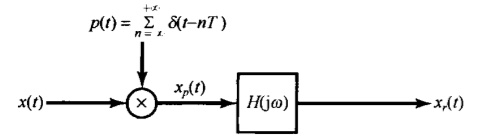
\includegraphics[scale=.3]{ss-c-f7-4a}
    	\end{center}
	和
    	\[
    	x_p(t)=\sum_n x(nT)\delta(t-nT)
    	\]
	有
    	\begin{align*}
        	x_r(t) & = x_p(t)*h(t) \\
			& = \int_R x_p(\tau)h(t-\tau)d\tau \\
			& = \int_R \sum_n x(nT)\delta(\tau-nT) h(t-\tau)d\tau \\
			& = \sum_n x(nT) \int_R \delta(\tau-nT) h(t-\tau)d\tau \\
			& = \sum_n x(nT) h(t-nT)
    	\end{align*}   
    \end{itemize}
  \end{frame} 

  %% PAGE
  \begin{frame}
    \frametitle{插值(interpolation)重建}
    \begin{itemize}
    \item 频率响应为$H(j\omega)$的理想低通滤波器
	    \begin{center}
    	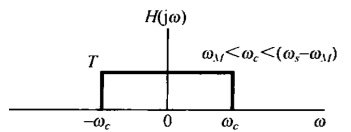
\includegraphics[scale=.3]{ss-c-f7-4d}
    	\end{center}
 	的单位冲激响应$h(t)$
	\[
		h(t)=\mathscr{F}^{-1}(H(j\omega))=\frac{\omega_c T sin(\omega_c t)}{\pi\omega_c t}
	\]
	因此
	\[
		x_r(t) = \frac{\omega_c T}{\pi} \sum_n x(nT)\frac{sin(\omega_c(t-nT))}{\omega_c (t-nT)}
	\]
    \end{itemize}
  \end{frame}   
  
  %% PAGE
  \begin{frame}
    \frametitle{插值(interpolation)重建}
    \begin{itemize}
    \item 取$\omega_c=\frac{\omega_s}{2}=\frac{\pi}{T}$
		\begin{align*}
			x_r(t) & = \frac{\omega_c T}{\pi} \sum_n x(nT)\frac{sin(\omega_c(t-nT))}{\omega_c (t-nT)} \\
		       	   & = \sum_n x(nT)sinc(\frac{t-nT}{T}), where \hspace{1mm} sinc(\theta)=\frac{sin(\pi \theta)}{\pi \theta}
		\end{align*}
	\item 上式被称为Shannon(香农)插值公式(1949年)
		\begin{center}
      	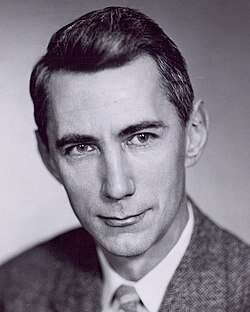
\includegraphics[scale=.3]{Claude_Shannon} \\
    	\href{https://en.wikipedia.org/wiki/Claude_Shannon}{Claude Shannon}   	
	\end{center}
    \end{itemize}
  \end{frame}   
  
    %% PAGE
  \begin{frame}
    \frametitle{插值(interpolation)重建}
    \begin{center}
      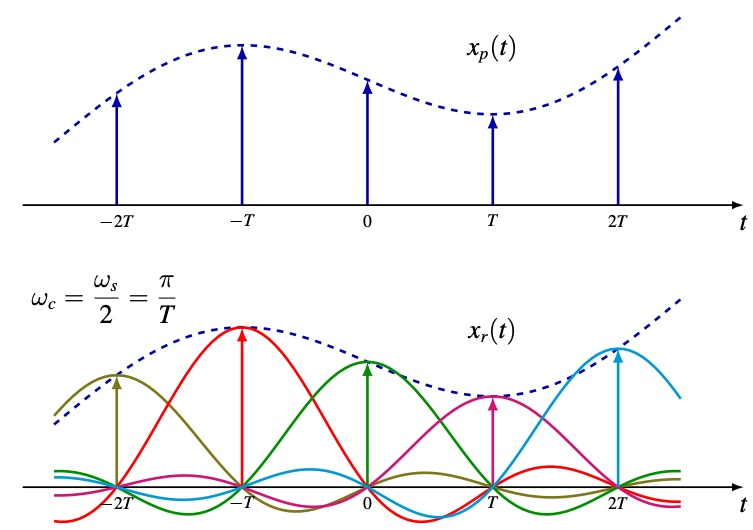
\includegraphics[scale=.4]{reconstruction}
    \end{center}
  \end{frame} 
  
    %% PAGE
  \begin{frame}
    \frametitle{奈奎斯特-香农采样定理}
	\begin{itemize}
	\item 联合奈奎斯特的采样定理和香农的插值重建公式,完成了信号的采样与重建
		\begin{itemize}
		\item 因此,奈奎斯特采样定理也被称为奈奎斯特-香农采样定理
		\end{itemize}
	\end{itemize}
  \end{frame}   
  
  %% PAGE
  \begin{frame}
    \frametitle{Questions}
    \begin{itemize}
    \item Any questions?
    \end{itemize}
    \begin{center}
      
\includegraphics[scale=.5]{question}
    \end{center}
  \end{frame} 

	\section{欠采样}
	
  %% PAGE
  \begin{frame}
    \frametitle{混叠}
    \begin{itemize}
    \item 当$\omega_s \leq 2\omega_M$时
    \[
    	X_p(j\omega)=\frac{1}{T}\sum_{k=-\infty}^{\infty} X(j(\omega-k\omega_s))
    \]
    中的求和项发生重叠,称这种现象为混叠(aliasing)。
    \begin{center}
      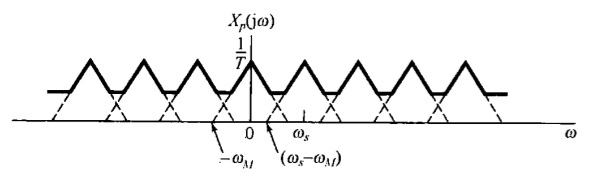
\includegraphics[scale=.5]{ss-c-f7-3d}
    \end{center}
    此时,尽管$x_r(nT)=x(nT), n=0, \pm1, \pm2, \hdots$,但一般$x_r(t) \neq x(t)$
    \end{itemize}
  \end{frame} 
  
  %% PAGE
  \begin{frame}
    \frametitle{例子}
	$cos(\omega_0 t + \phi) = \frac{1}{2}e^{j(\omega_0 t+ \phi)}+\frac{1}{2}e^{-j(\omega_0 t+ \phi)}	$

    \begin{center}
    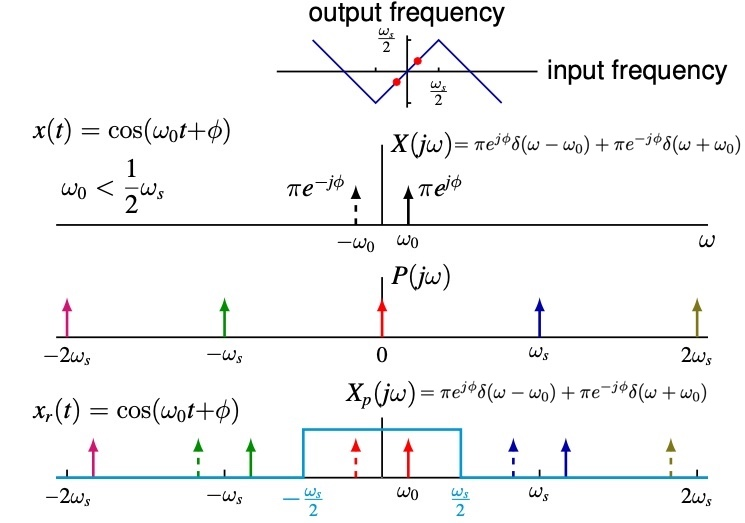
\includegraphics[scale=.42]{aliasing-example-1}
    \end{center}

  \end{frame}   

  %% PAGE
  \begin{frame}
    \frametitle{例子}
	$cos(\omega_0 t + \phi) = \frac{1}{2}e^{j(\omega_0 t+ \phi)}+\frac{1}{2}e^{-j(\omega_0 t+ \phi)}	$

    \begin{center}
    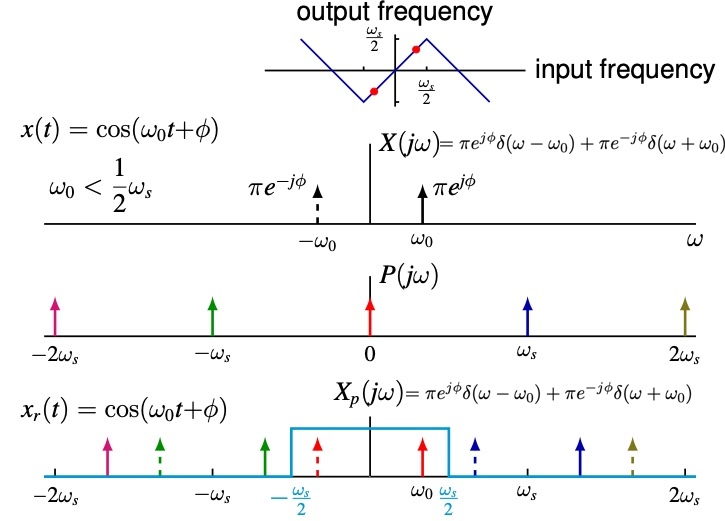
\includegraphics[scale=.42]{aliasing-example-2}
    \end{center}

  \end{frame}   
  
  %% PAGE
  \begin{frame}
    \frametitle{例子}
	$cos(\omega_0 t + \phi) = \frac{1}{2}e^{j(\omega_0 t+ \phi)}+\frac{1}{2}e^{-j(\omega_0 t+ \phi)}	$

    \begin{center}
    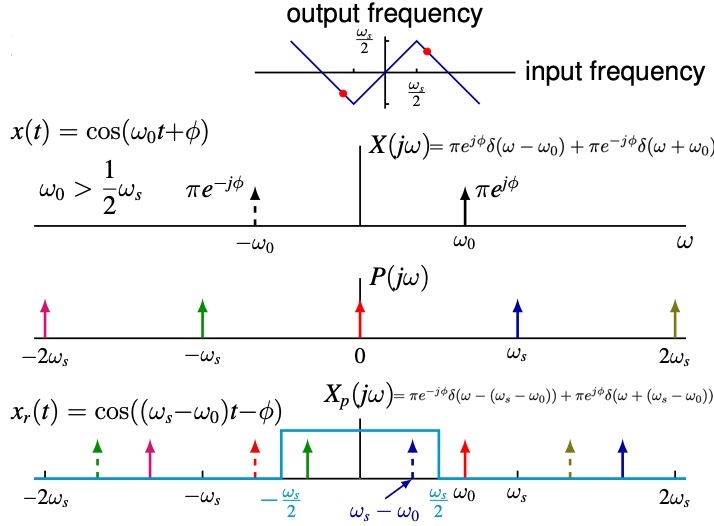
\includegraphics[scale=.42]{aliasing-example-3}
    \end{center}

  \end{frame}   
  
  %% PAGE
  \begin{frame}
    \frametitle{例子}
	$cos(\omega_0 t + \phi) = \frac{1}{2}e^{j(\omega_0 t+ \phi)}+\frac{1}{2}e^{-j(\omega_0 t+ \phi)}	$

    \begin{center}
    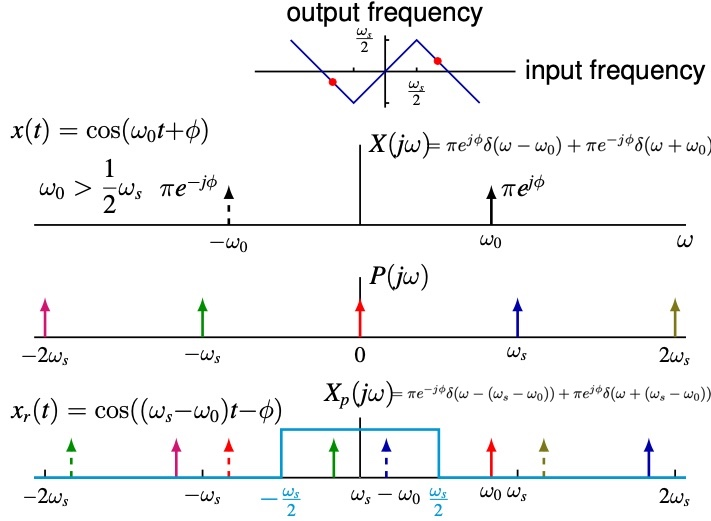
\includegraphics[scale=.42]{aliasing-example-4}
    \end{center}

  \end{frame}       
    	
  %% PAGE
  \begin{frame}
    \frametitle{例子}

	\begin{itemize}
	\item 也就是说,固定采样频率$\omega_s$,随着信号频率$\omega_0$的增加,频率发生了折叠(wrap)
	\end{itemize}

  \end{frame}   
	
  %% PAGE
  \begin{frame}
    \frametitle{Questions}
    \begin{itemize}
    \item Any questions?
    \end{itemize}
    \begin{center}
      
\includegraphics[scale=.5]{question}
    \end{center}
  \end{frame} 
  
	\section{量化}

\ifxetexorluatex\else
\end{CJK*}
\fi
\end{document}

%%% Local Variables: 
%%% mode: latex
%%% TeX-master: t
%%% End: 
